%\documentstyle[10pt,twoside]{article}
%\documentstyle[twoside]{article}
\documentclass[twoside]{article}
\setlength{\oddsidemargin}{0.25 in}
\setlength{\evensidemargin}{-0.25 in}
\setlength{\topmargin}{-0.6 in}
\setlength{\textwidth}{6.5 in}
\setlength{\textheight}{8.5 in}
\setlength{\headsep}{0.75 in}
\setlength{\parindent}{0 in}
\setlength{\parskip}{0.1 in}

\usepackage{graphicx}
\usepackage{amsmath}
\usepackage{float}
\usepackage{url}


%
% The following commands sets up the lecnum (lecture number)
% counter and make various numbering schemes work relative
% to the lecture number.
%
\newcounter{lecnum}
\renewcommand{\thepage}{\thelecnum-\arabic{page}}
\renewcommand{\thesection}{\thelecnum.\arabic{section}}
\renewcommand{\theequation}{\thelecnum.\arabic{equation}}
\renewcommand{\thefigure}{\thelecnum.\arabic{figure}}
\renewcommand{\thetable}{\thelecnum.\arabic{table}}
\newcommand{\dnl}{\mbox{}\par}

%
% The following macro is used to generate the header.
%
\newcommand{\lecture}[4]{
   \pagestyle{myheadings}
   \thispagestyle{plain}
   \newpage
   \setcounter{lecnum}{#1}
   \setcounter{page}{1}
   \noindent
   \begin{center}
   \framebox{
      \vbox{\vspace{2mm}
    \hbox to 6.28in { {\bf CMPSCI~677~~~Operating Systems
                        \hfill Spring 2017} }
       \vspace{4mm}
       \hbox to 6.28in { {\Large \hfill Lecture #1: #2  \hfill} }
       \vspace{2mm}
       \hbox to 6.28in { {\it Lecturer: #3 \hfill Scribe: #4} }
      \vspace{2mm}}
   }
   \end{center}
   \markboth{Lecture #1: #2}{Lecture #1: #2}
   \vspace*{4mm}
}

%
% Convention for citations is authors' initials followed by the year.
% For example, to cite a paper by Leighton and Maggs you would type
% \cite{LM89}, and to cite a paper by Strassen you would type \cite{S69}.
% (To avoid bibliography problems, for now we redefine the \cite command.)
%
\renewcommand{\cite}[1]{[#1]}

% \input{epsf}

%Use this command for a figure; it puts a figure in wherever you want it.
%usage: \fig{NUMBER}{FIGURE-SIZE}{CAPTION}{FILENAME}
\newcommand{\fig}[4]{
            %\vspace{0.2 in}
            \centerline{\includegraphics[scale=#2]{#4}}
            \begin{center}
            Figure \thelecnum.#1:~#3
            \end{center}
    }

% Use these for theorems, lemmas, proofs, etc.
\newtheorem{theorem}{Theorem}[lecnum]
\newtheorem{lemma}[theorem]{Lemma}
\newtheorem{proposition}[theorem]{Proposition}
\newtheorem{claim}[theorem]{Claim}
\newtheorem{corollary}[theorem]{Corollary}
\newtheorem{definition}[theorem]{Definition}
\newenvironment{proof}{{\bf Proof:}}{\hfill\rule{2mm}{2mm}}

% Some useful equation alignment commands, borrowed from TeX
\makeatletter
\def\eqalign#1{\,\vcenter{\openup\jot\m@th
  \ialign{\strut\hfil$\displaystyle{##}$&$\displaystyle{{}##}$\hfil
      \crcr#1\crcr}}\,}
\def\eqalignno#1{\displ@y \tabskip\@centering
  \halign to\displaywidth{\hfil$\displaystyle{##}$\tabskip\z@skip
    &$\displaystyle{{}##}$\hfil\tabskip\@centering
    &\llap{$##$}\tabskip\z@skip\crcr
    #1\crcr}}
\def\leqalignno#1{\displ@y \tabskip\@centering
  \halign to\displaywidth{\hfil$\displaystyle{##}$\tabskip\z@skip
    &$\displaystyle{{}##}$\hfil\tabskip\@centering
    &\kern-\displaywidth\rlap{$##$}\tabskip\displaywidth\crcr
    #1\crcr}}
\makeatother

% **** IF YOU WANT TO DEFINE ADDITIONAL MACROS FOR YOURSELF, PUT THEM HERE:



% Some general latex examples and examples making use of the
% macros follow.

\begin{document}

%FILL IN THE RIGHT INFO.
%\lecture{**LECTURE-NUMBER**}{**DATE**}{**LECTURER**}{**SCRIBE**}
\lecture{25}{April 30}{Prashant Shenoy}{\textbf{Daniel Saunders}}

\section{Distributed Security}

\subsection{Authentication using public keys}

AP 4.0 uses symmetric keys for authenticantion. \textbf{Question}: can we use public keys? \textit{symmetry}: DA(EA($n$)) = EA(DA($n$)).

\textbf{AP 5.0}: \\
\hspace*{1.0cm} A to B: msg = ``I am A'' \\
\hspace*{1.0cm} B to A: once in a lifetime value $n$ \\
\hspace*{1.0cm} A to B: msg = DA($n$) \\
\hspace*{1.0cm} B computes: If EA(DA($n$)) = $n$ \\
\hspace*{2.0cm} then A is verified \\
\hspace*{2.0cm} else A is fradulent \\

\subsection{Man-in-the-middle attack}

Trudy impersonates as Alice to Bob and as Bob to Alice.

\begin{center}
\begin{tabular}{ccccc}
 Alice &            & Trudy &            & Bob \\
       & ``I am A'' &       & ``I am A'' &     \\
       &            &       & nonce $n$  &     \\
       &            &       & DT($n$)    &     \\
       &            &       & send me ET &     \\
       & nonce $n$  &       &            &     \\
       & DA($n$)    &       &            &     \\
       & send me EA &       &            &     \\
       & EA         &       &            &     \\
\end{tabular}
\end{center}

Bob sends data using ET, and Trudy decrypts and forwards it using EA (Trudy \textit{transparently} intercepts every message).

\subsection{Digital signatures using public keys}

\textbf{Goals of digital signatures}:

\begin{itemize}
\item Sender cannot repudiate message never sent (``I never sent that'').
\item Receiver cannot fake a received message.
\end{itemize}

Suppose A wants B to ``sign'' a message M.

B send DB(M) to A \\
A computes if EB(DM(A)) = M \\
\hspace*{1.0cm} then B has signed M \\

\textbf{Question}: Can B plausibly deny having sent M?

\subsection{Message digests}

Encypting and decrypting entire messages using digital signatures is computationally expensive. Routers routinely exchange data, which do not need encryption, but do require authentication and to verify that data hasn't changed.

A message digest is a compact summary of a message, like a checksum. A has function $H$ converts a variable length string to a fixed length hash value. The user will then digitally sign $H(M)$, and send both $M$ and $DA(H(M))$. The receiver can verify who sent the message and that it has been changed.

\textbf{Important property of $H$}: Given a digest $x$, it is infeasible to find a message $y$ for which $H(y) = x$. Also, it is infeasible to find any two messages such that $H(x) = H(y)$ (hash collision). If the hash function $H$ satisfies this property, then this scheme is much more efficient than digital signatures with public keys: we need only encrypt the fixed-length hash value $H(M)$, typically much shorter than $M$.

\subsection{Hash functions: MD5}

MD5 takes an arbitrarily-sized objects, splits it into smaller chunks, and hash each of the chunks. This method is recursed until we have a fixed-sized hash value.

\begin{figure}[h]
\centering
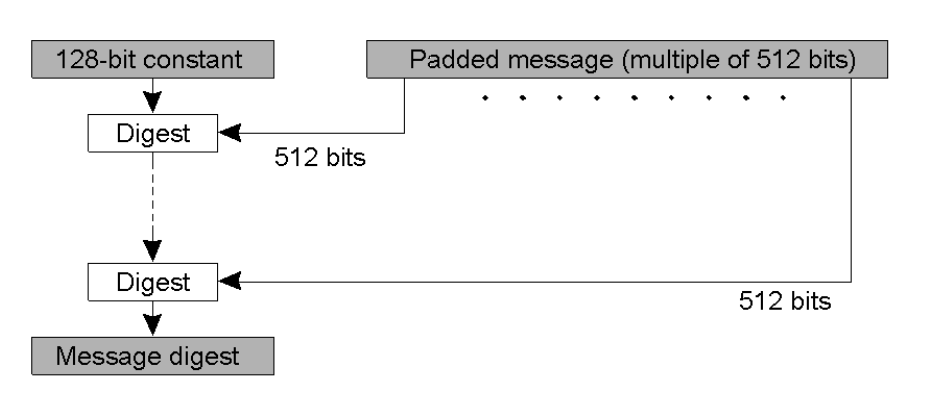
\includegraphics[width=0.8\textwidth]{md5.png}
\caption{The structure of MD5.}
\end{figure}

\subsection{Hash functions: SHA}

MD5 is not secure anymore. Secure Hash Algorithms (SHA) hash functions:

\begin{itemize}
\item SHA-1: 160-bit function that resembles MD5.
\item SHA-2: family of two hash functions (SHA-256 and SHA-512).
\item Developed by NIST and NSA.
\end{itemize}

Let's say you have a hashed value $h$, and you want to know the original message $m$ such that $H(m) = h$. How can we find out $m$? We could carry out a dictionary attack, in which we try all $m'$ in some ``dictionary'' and compute $H(m')$. If any such $m'$ produces $H(m') = h$, then $m' = m$. Clearly, the longer the message, the more time required by this brute-force attack.

\subsection{Symmetric key exchange: trusted server}

\textbf{Problem}: How do distributed entities agree on a key?

This is the problem of key distribution. If keys are comprised, than anyone may use your key to decrypt your messages. We need a secure method of key exchange; it must be just as strong as your encryption algorithm itself.

\textbf{Assume}: Each entity has its own single key, which only it and a trusted server know.

\textbf{Server}:

\begin{itemize}
\item Will generate a one-time session key (symmetric) that A and B use to encrypt all communication.
\item Will use A and B's single keys to communicate session key to A and B.
\end{itemize}

\subsection{Key exchange: key distribution center}

Trusted third party as the key distribution center. Alice sends a message to the KDC saying ``I'm Alice, and I want to communicate with Bob; please generate a key''. The KDC generates a random session key, encrypts it with Alice's public key, and sends it back to Alice. The KDC will send the same key to Bob, encryped with Bob's public key.

\begin{figure}[H]
\centering
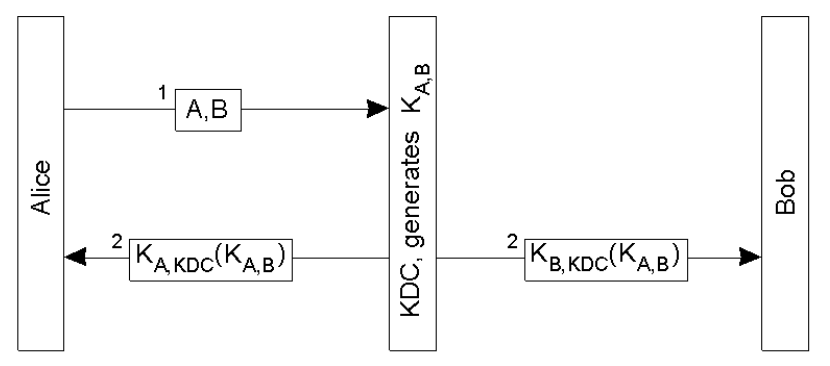
\includegraphics[width=0.6\textwidth]{kdc.png}
\caption{The principles of using a KDC.}
\end{figure}

\subsection{Authentication using a key distribution center}

\textbf{Pictured below}: Same technique as before, but the KDC does not actually send a message to Bob. Messages are sent from Alice to Bob.

\begin{figure}[H]
\centering
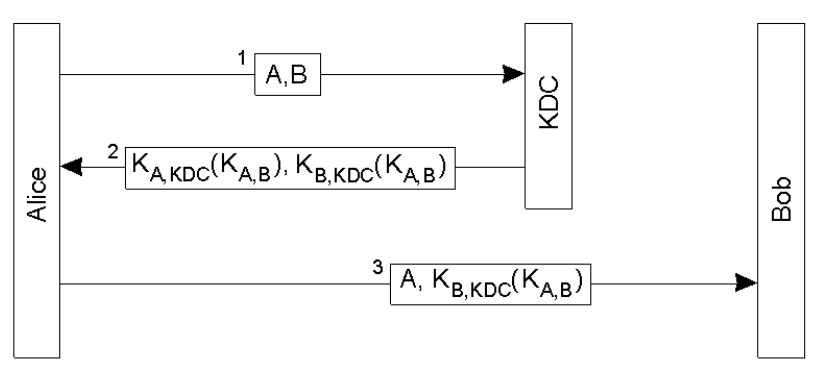
\includegraphics[width=0.6\textwidth]{kdc2.png}
\caption{Using a ticket and letting Alice set up a connection to Bob.}
\end{figure}

\textbf{Pictured below}: The Needham-Schroeder authentication protocol uses a session key as well as a nonce (once-in-a-lifetime integer) for Alice to talk to the KDC. A second nonce is generated by Alice to begin communicating with Bob. Bob will generate a nonce as well and send it and the nonce from Alice back to Alice. The nonces are used as an extra validation step.

\begin{figure}[H]
\centering
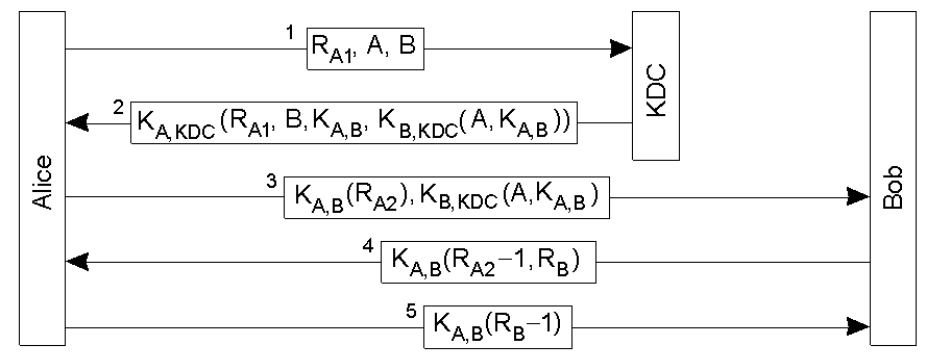
\includegraphics[width=0.6\textwidth]{kdc3.png}
\caption{The Needham-Schroeder authentication protocol.}
\end{figure}

\subsection{Public key exchange}

There is no KDC in this protocol; public and private keys are used only. This protocol assumes we have a secure way of getting someone's public key before communicating with them. Alice sends a nonce to Bob, which is encrypted by Alice with Bob's public key. Bob decrypts it, sends it back, sends a new nonce and session key back (all of this is encrypted with Alice's public key). Alice decrypts this message, and sends back Bob's generated nonce for validation purposes.

\begin{figure}[H]
\centering
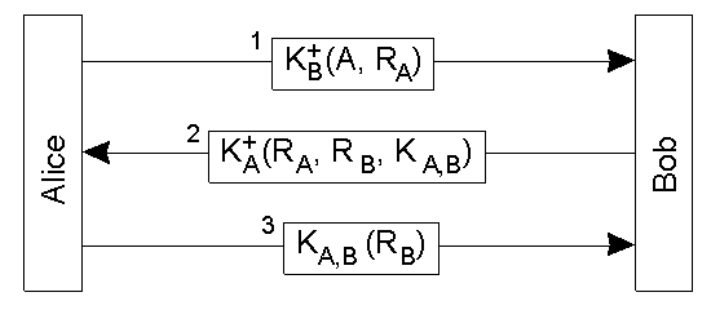
\includegraphics[width=0.6\textwidth]{public_key_exchange.png}
\caption{Mutual authentication in a public-key cryptosystem.}
\end{figure}

Public key retrieval is subject to man-in-the-middle attacks if public keys aren't shared securely. We can use a trusted third party in order to distributed public keys securely. This third party will issue ``certificates'', public keys of servers which are signed by the trusted third party. All servers have the trusted server's encryption key. Suppose that A wants to send B a message using B's ``public'' key; A can accomplish this by using certificates from the trusted third party. Certificates may be revoked.

\begin{figure}[H]
\centering
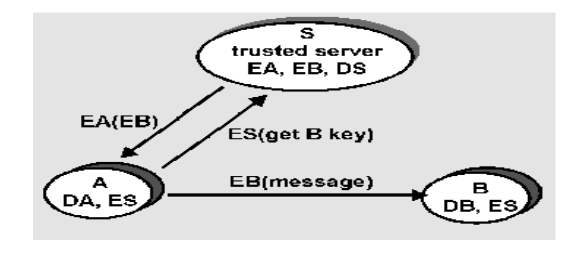
\includegraphics[width=0.5\textwidth]{pke_trusted.png}
\caption{Public key exchange: trusted server.}
\end{figure}

\subsection{Security in enterprises}

\begin{itemize}
\item In the multi-layered approach to security, Security functionality is spread across multiple components.
\item Firewalls
\item Deep packet inspection
\item Virus and email scanning
\item VLANS
\item Network radius servers
\item Securing WiFi
\item VPNs
\item Securing services using SSL, certificates, kerberos
\end{itemize}

Distributed systems security or network security are very complex problems. There are many layers of security protections that are deployed, and things get complicated fast. Companies typically get hacked because there is a small issue with one or more of the security items listed above.

\subsection{Security in internet services}

How can we secure internet services?

\begin{itemize}
\item Websites

\begin{itemize}
\item Ensure all connections between browser and server are encrypted.
\item Authenticate user (username and password checks).
\item Use techniques like CAPTCHAs to prevent scripts from launching attacks.
\end{itemize}

\item Challenge-response authentication

\begin{itemize}
\item Push a one-time key to a user's phone to enter for further authentication.
\end{itemize}

\item Two-factor authentication

\begin{itemize}
\item Password and mobile phone (gmail).
\end{itemize}

\item One-time passwords
\item Online merchant payments: paypal, amazon payments, google checkouts

\end{itemize}

\subsection{Firewalls}

A firewall is a machine that sits on the boundary of the internal (e.g., home WiFi) and external networks (e.g., the Internet). All traffic between the internal and external networks must pass through the firewall, which has a pre-configured set of packet-filtering rules. If a packet matches one of the firewall's rules, it is allowed to pass; otherwise, it is dropped. 

\begin{figure}[H]
\centering
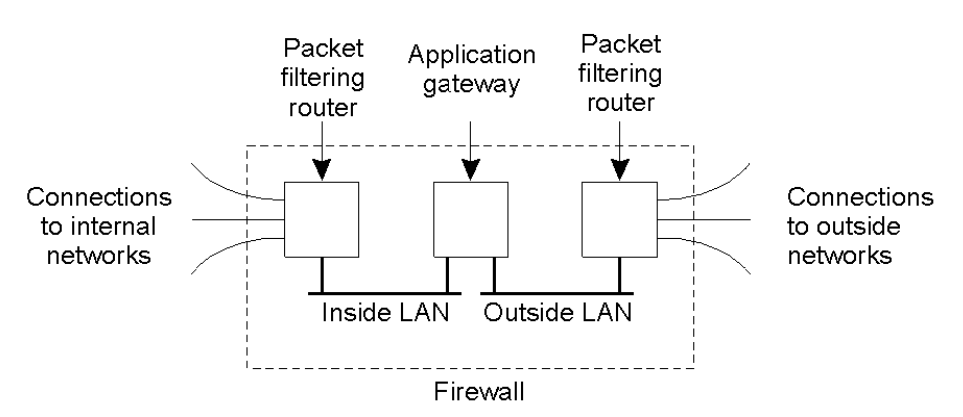
\includegraphics[width=0.7\textwidth]{firewall.png}
\caption{A common implementation of a firewall.}
\end{figure}

\subsection{Secure email}

\begin{itemize}
\item Requirements

\begin{itemize}
\item Secrecy
\item Sender authentication
\item Message integrity
\item Receiver authentication
\end{itemize}

\item Secrecy

\begin{itemize}
\item Can use public keys to encrypt messages (this is inefficient for long messages because public keys are very long).
\item Use shorter, message-specific symmetric keys

\begin{itemize}
\item Alice generates symmetric key $K$
\item Encrypt message $M$ with $K$
\item Encrypt $K$ with $E_B$
\item Send $K(M), E_B(K)$
\item Bob decrypts using his private key, gets $K$, and decrypts $K(M)$
\end{itemize}

\end{itemize}

\item Authentication and Integrity (without secrecy)

\begin{itemize}
\item Alice applies has function $H$ to $M$ ($H$ can be MD5 or SHA)
\item Creates a digital signature $D_A(H(M))$ 
\item Send $M, D_A(H(M))$ to Bob
\end{itemize}

\item Putting it all together

\begin{itemize}
\item Compute $H(M), D_A(H(M))$
\item $M' = \{M, D_A(H(M)) \}$
\item Generate symmetric key $K$, compute $K(M')$
\item Encrypt $K$ as $E_B(K)$
\item Send $K(M'), E_B(K)$
\end{itemize}

\item Used in PGP (pretty good privacy)

\end{itemize}

\subsection{Secure sockets layer (SSL)}

SSL (developed by NetScape) provides data encryption and authentication between web servers and clients. It lies above the transport layer. It is used for internet commerce, secure mail access (IMAP), and more. Features include: SLL server authentication, encrypted SSL sessions, and SSL client authentication.

It uses the HTTPS protocol instead of HTTP. The browsers sends the first message to the server saying it can support some version of SSL, and the server responds with its supported version of SSL, as well as a certificate (server's RSA public key encrypted by a trusted third party's (certification authority) private key). The browser generates a session key $K$, and encrypts the key with $E_S$, the public key of the server sent in the certificate. The browser sends ``future messages will be encrypted'' and $K(M)$ to the server, and the server responds with the same. The SSL session then begins.

\section{Electronic payment systems}

Payment systems based on direct payments between customer and merchant. 

\begin{figure}[H]
\centering
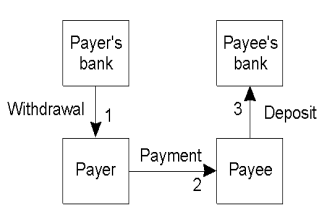
\includegraphics[width=0.35\textwidth]{eps1.png}
\centering
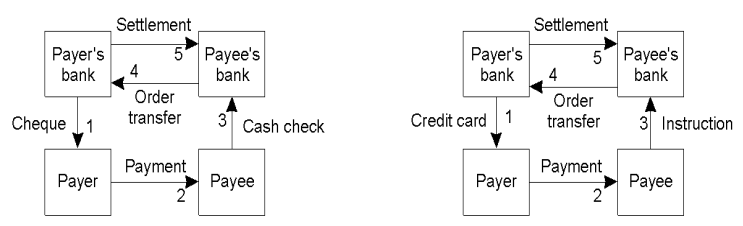
\includegraphics[width=0.7\textwidth]{eps2.png}
\caption{(a) Paying in cash; (b) Using a check; (c) Using a credit card.}
\end{figure}

\subsection{E-cash}

We want to use a digital form of cash which has anonymity properties. Users may generate ``coins'', an integer token, which are ``blinded'' (hide the sequence number of currency to the bank; this prevents the bank from tracking how they are spent), and request the bank to ``sign'' it. The signed coin is unblinded, and subsequently used as a currency, which are check for validity (valid coins have not already been spent) with the bank before transactions can take place.

\begin{figure}[H]
\centering
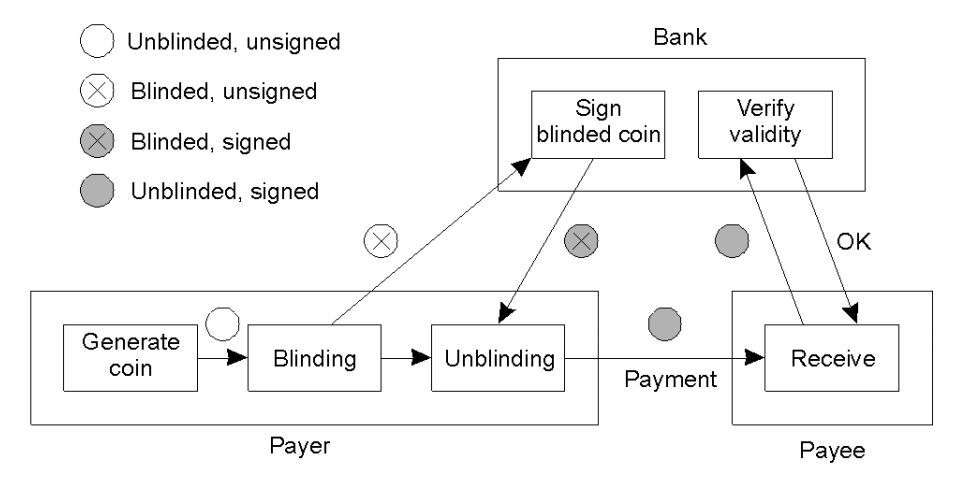
\includegraphics[width=0.8\textwidth]{ecash.png}
\caption{Illustration of E-cash.}
\end{figure}

\subsection{Bitcoin}

Bitcoin is a digital currency which uses peer-to-peer (P2P) transactions so as to avoid using a central bank or organization as the middle man (decentralized).

\begin{figure}[H]
\centering
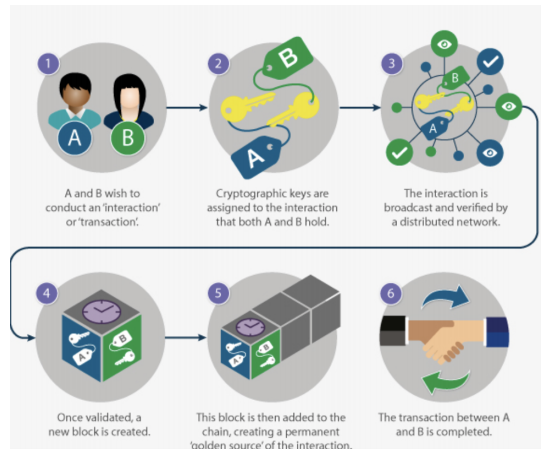
\includegraphics[width=0.7\textwidth]{bitcoin.png}
\caption{How Bitcoin works.}
\end{figure}

\subsection{Blockchain: distributed ledger}

Blockchain is a distributed database (ledger) which records every transactions that goes through the system. It uses a generic protocol for transactions based on public key cryptography. All the currency exchanged using the system and how much currency is owned by each person is publicly available. Transactions are signed by private keys and added into the ledger. The blockchain is massively replicated and shared using the P2P file sharing protocol. Special nodes called ``miners'' update the blockchain by appending blocks of multiple transactions. All nodes perform validation of transactions. Miner nodes perform ``settlement'' using a distributed consensus protocol.

\begin{figure}[H]
\centering
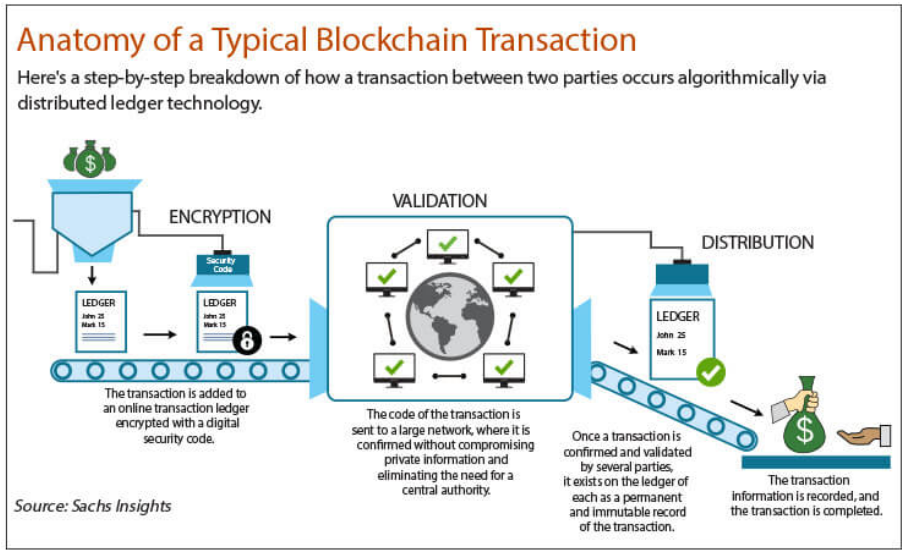
\includegraphics[width=0.7\textwidth]{blockchain.png}
\caption{How blockchain works.}
\end{figure}

\end{document}